


%%%%%%%%%%%%%%%%%%%%%%%%%%%
\chapter{ OMSN routing protocol simulator}
\label{OPS}
%%%%%%%%%%%%%%%%%%%%%%%%%%%

\noindent The Opportunistic Networking Environment (ONE) \cite{C35} is a simulator designed for evaluating DTN routing and application protocols. Researchers can import real-world map into the simulator so that hosts walk along streets and roads in the simulator. The movement model of hosts can be defined by researchers, which enables researchers to evaluate the performance of their protocols in different scenarios. The User Interface of the ONE is also friendly, where researchers can observe the movement of all hosts. When a round of experiment ends, ONE outputs the results to a defined file. The simulator can also execute in console mode, which allows a higher experiment speed.

The ONE is an excellent simulator for DTN research, while it has its own weakness. The way that ONE estimates the distance between two hosts is not thorough, which may lead to inaccurate results. When a host broadcasts a message, only the hosts which are in its communication radius should receive the message. If the simulator cannot give the accurate set of hosts which can receive the message, the experiment result is not reliable. Although we can avoid this problem by setting parameters carefully, this problem cannot be completely ignored. Besides, some movement models need to calculate shortest path several times, which may require several seconds. Even though that is not a long time, it can slow down the experiment speed significantly as the total time of a round of experiment is about 10-20 seconds. 

In this chapter, we introduce two major algorithms used in our new ORS simulator. The vertex reduce algorithm is used for simplifying the input of the all-pair shortest path algorithm, so that the simulator can initialize quickly. The finding nodes algorithm is used to find users which are in the communication radius of a given user.


\section{ Vertex Reduction Algorithm}

\noindent Movement of network nodes is a significant factor in the performance of DTNs. To evaluate the performance of different DTN protocols, researchers have presented different kinds of movement models, like in \cite{C32}. Since shortest path algorithm is an essential and time-cost part of creating many movement models, it is an important aspect to optimize the time-cost for simulators, calculating the all-pairs shortest paths in the entire map.

The best known non-negative edge weight undirected map all-pairs shortest path algorithm \cite{C33} has a complexity $O\left(n^2{\mathrm{log} n\ }\right)$, which is still expensive when \textit{n} is huge. For most real-world city maps, there are thousands of points in a single square kilometer. Since a ten-square kilometers map is reasonable for a DTN protocol evaluation, a simulator must cut down the time spent in calculating all-pairs shortest paths to speed up the experiment.

Real-world map developers often use short straight lines to present curves, like in \cite{C34}, so that a several-meters curves may contain tens of points. It is obvious that we do not need to calculate shortest path for every one of these points. In this chapter, we present an Vertex Reduction Algorithm (VRA) to reduce the number of points before the use of the shortest path algorithm. The basic idea is that VRA removes all points whose degrees are less than 3 from the map, while keeping the result of all-pairs shortest path algorithm correct.

The rest of this chapter is organized as follows. Section \ref{subsecIVRV} presents some basic definitions and lemmas. The process of VRA is described in Section \ref{subsecVR} and Section \ref{subsecAssVer}.



\subsection{ Ignorable Vertex and Reserved Vertex}\label{subsecIVRV}

\noindent Vertices in the graph are considered ignorable and/or reserved (definition follows). In each iteration of VRA, we remove the ignorable vertex from the graph, while the reserved vertices compose a new graph.

\textit{Definition} \textit{1}: The vertex whose degree is larger than 2 is the \textit{reserved} vertex (denoted by $R$).

\textit{Definition} \textit{2}: The vertex whose degree is smaller than or equal to 2 is called the \textit{ignorable} vertex (denoted by $G$).

\textit{Definition} \textit{3}: If two reserved vertices (e.g. $R_1,R_2$) are connected by a sequence of ignorable vertices (e.g. $G_1,G_2,\mathrm{\cdots },G_n$), then the sequence from $R_1$ to $R_2$ (i.e., $R_1,G_1,G_2,\mathrm{\cdots },G_n,R_2$) is a \textit{line-segment} (denoted by $LS$). 

A reserved vertex can belong to different line-segments, while an ignorable vertex belongs to a unique line-segment. Both the reserved vertex and the ignorable vertex are called vertices ($V$)\textit{}

\textit{Definition} \textit{4}: The shortest route between two vertices inside a \textit{segment-line} is called the \textit{inner shortest path} ($SPI$). 

Let ${SPI}\left(V_i,V_j\right)$ denote the inner shortest path between two vertices (i.e. $V_i,V_j$) inside a \textit{segment-line}.

\textit{Lemma} \textit{1}: If two vertices (i.e. $V_i$, $V_j$; $i<j$) are in the same line-segment, the shortest path between them is

\begin{equation} \label{GrindEQ__VRShortestInner} 
{SP}\left(V_i,V_j\right)={min}\left\{SPI\left(V_i,V_j\right),SPI\left(R_1,V_i\right)+SPI\left(V_j,R_2\right)+SP\left(R_1,R_2\right)\right\}
\end{equation}

\textit{Proof}: \textit{Lemma} \textit{1} is shown in Figure \ref{fig:ShortestPathOnASingleSegment}. We assume that there is a path (e.g., $V_i-V_x-V_j$) whose length is smaller than or equal to Equation \ref{GrindEQ__VRShortestInner} between $V_i$, $V_j$, where $V_x$ is a vertice in the \textit{segment-line} including $V_i$, $V_j$.

\begin{figure} [hbtp]
  \centering 
  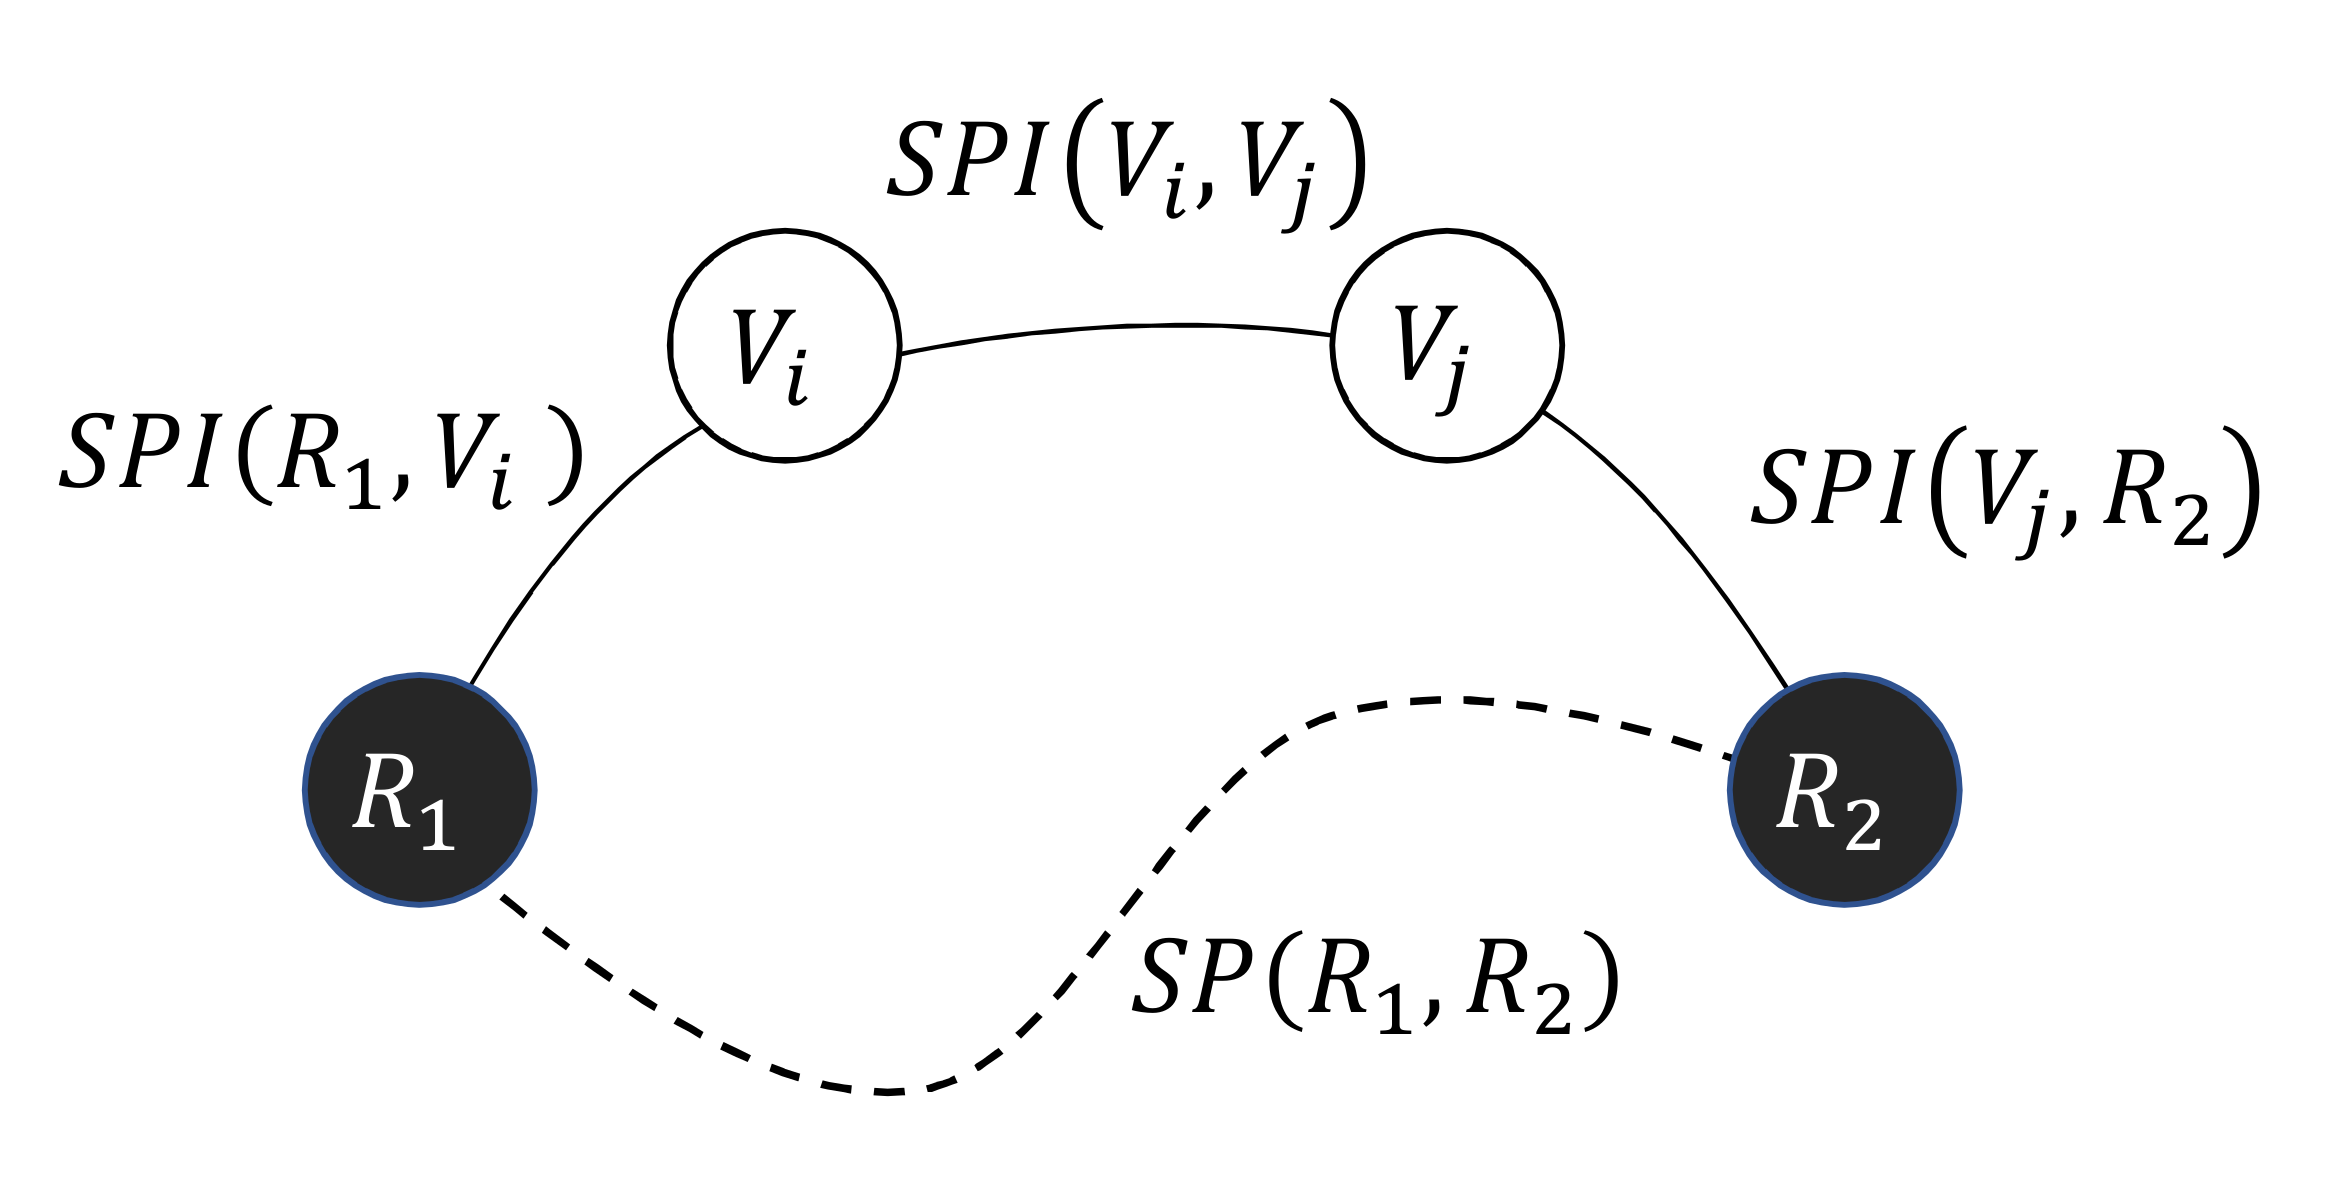
\includegraphics[height=1.5in]{figures/ShortestPathOnASingleSegment.png}
  \caption{Shortest Path On A Single Segment-Line} 
  \label{fig:ShortestPathOnASingleSegment} %% label for entire figure 
\end{figure}

Case 1: $V_x$ is between $V_i$ and $V_j$. The length of the path $V_i-V_x-V_j$ must be equal to $SPI\left(V_i,V_j\right)$ or there must be duplicated vertices on the path.

Case 2: $V_x$ is between $R_1$ and $V_i$ or between $V_j$ and $R_2$. $V_i-V_j$ should not be a part of the path or $V_i-V_j$ could be the shortest path. Then the path $V_i-R_1-R_2-V_j$ must be a part of $V_i-V_x-V_j$ because $R_1$ and $R_2$ are entrances of the \textit{segment-line}.

Since an all-pairs SPI has a complexity equal to or smaller than $O\left(n\right)$ and the \textit{n} here is much fewer than the number of points on the entire map, the time-cost for SPI is ignorable comparing to the time-cost of the entire map all-pairs shortest path calculation.

\textit{Lemma 2}: We assume that there are two different line-segments 

\noindent ${LS}_i=\left\{R_{i1},G_{i1},G_{i2},\cdots,G_{in},R_{i2}\right\}$ and ${LS}_j=\left\{R_{j1},G_{j1},G_{j2},\cdots,G_{jm},R_{j2}\right\}$. We pick a vertex $V_i$ from $LS_i$ and a vertex $V_j$ from $LS_j$, then the shortest path between $V_i$ and $V_j$ is 

\begin{equation} \label{GrindEQ__VRShortestOutside} 
\begin{split}
SP\left(V_i,V_j\right)=min\{SP\left(V_i,R_{i1},R_{j1},V_j\right),SP\left(V_i,R_{i2},R_{j1},V_j\right), \\
SP\left(V_i,R_{i1},R_{j2},V_j\right),SP\left(V_i,R_{i2},R_{j2},V_j\right)\}
\end{split}
\end{equation}

where $\mathrm{SP}\left(V_i,R_{ia},R_{jb},V_j\right)=\mathrm{SP}\left(V_i,R_{ia}\right)+\mathrm{SP}\left(R_{ia},R_{jb}\right)+\mathrm{SP}\left(R_{jb},V_j\right)$. Here $V_i$ and $R_{ia}$ are in the same line-segment, so we can use Lemma 1 to calculate $\mathrm{SP}\left(V_i,R_{ia}\right)$, so does $\mathrm{SP}\left(R_{jb},V_j\right)$. The $SP\left(R_{ia},R_{jb}\right)$ is the only part we need to calculate using all-pair shortest path algorithms. We should notice that $R_{ia}$ and $R_{jb}$ could be the same vertex, but it does not make any difference to the lemma.

\textit{Proof}: Since $V_i$ and $V_j$ are not in the same \textit{segment-line}, there must be one or more reserved vertices on their shortest path. On $V_i$'s side, one of $R_{i1}$ and $R_{i2}$ must be on the shortest path. One of $R_{j1}$ and $R_{j2}$ should be on that shortest path, either. We assume that $R_{iu}$ and $R_{jv}$ are on the shortest path between $V_i$ and $V_j$, then a shortest path between $R_{iu}$ and $R_{jv}$ should be a part of that path.


\subsection{ Vertex Reduction}\label{subsecVR}

\noindent VRA iteratively removes ignorable vertices from the graph until only reserved vertices remain. In each iteration, we remove all ignorable vertices from the graph but keep the edges. If there is more than one route between a pair of reserved vertices, we keep the shortest one and remove others. 


\subsubsection{ Remove Ignorable Vertices}\label{subsubsec_RIV}

\noindent Since the degree of ignorable vertices is no more than 2, an ignorable vertex has only 0, 1 or 2 neighbours. In the case of 0 or 1 neighbour, we simply delete the ignorable vertex; if it has two neighbours, we connect its two neighbours before it is removed, as shown in Figure \ref{fig:RemoveIgnorableVertices}. When we remove an ignorable vertex, the weight of the line which connects its two neighbours is equal to the sum of its recent two lines' weights (i.e., $W_l+W_r$). After we remove all ignorable vertices in a line-segment, the two reserved vertices at the end of the line-segment are connected with a line directly, whose weight is the sum of all the intermediate ones' (i.e., $W_1+W_2+W_3+W_4$).

\begin{figure} [hbtp]
  \centering 
  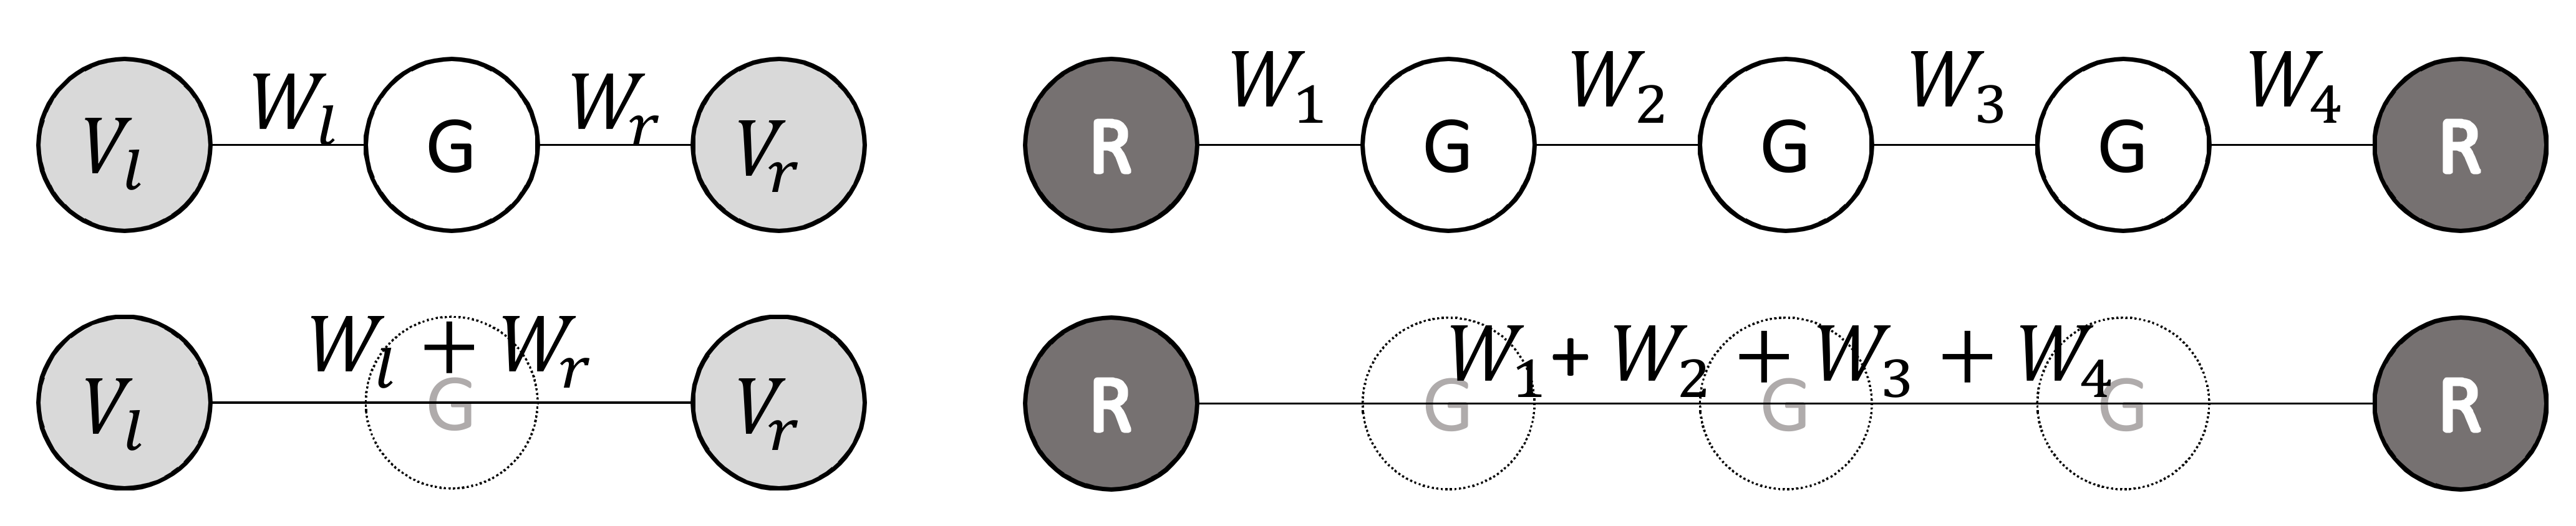
\includegraphics[height=1.2in]{figures/F51RemoveIgnorableVertices.png}
  \caption{Remove Ignorable Vertices} 
  \label{fig:RemoveIgnorableVertices} %% label for entire figure 
\end{figure}

\subsubsection{ Remove Redundant Connections}\label{subsubsec_RRC}

\noindent After we remove all ignorable vertices, all the reserved vertices are connected directly. However, it is possible that there are several connections between a pair of reserved vertices. Since the shortest route between a pair of neighbouring vertices makes other longer ones redundant, we remove all routes except the shortest one, as shown in Figure \ref{fig:F52TidyReservedConnections}. We assume that $W_2$ is the shortest line among three connections, when $W_1$ and $W_3$ are removed.

\begin{figure} [hbtp]
  \centering 
  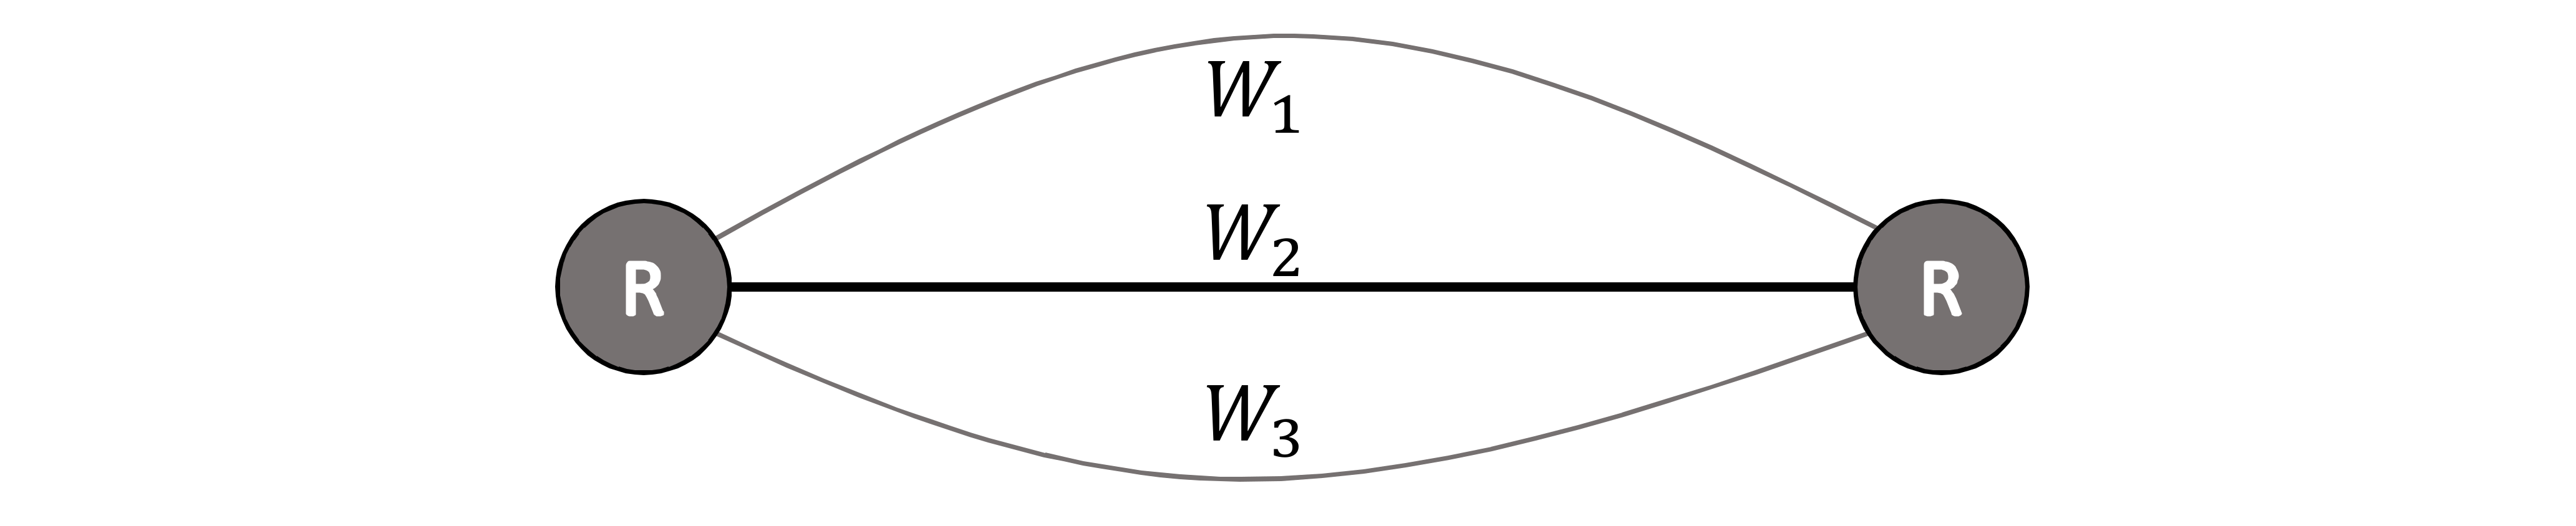
\includegraphics[height=1.2in]{figures/F52TidyReservedConnections.png}
  \caption{Tidy Reserved Connections} 
  \label{fig:F52TidyReservedConnections} %% label for entire figure 
\end{figure}

\subsubsection{ Iterations}

The process is shown in Algorithm \ref{AlgVerRed}. The input of the algorithm is the original entire map, which is called ${Graph}_0$. In the \textit{i}${}^{th}$ iteration, VRA makes a copy of ${Graph}_i$ as ${Graph}_{i+1}$. If $i>0$, the ${Graph}_i$ is the output of the previous (i.e., ${\left(i-1\right)}^{th}$) iteration. VRA removes all ignorable vertices in the ${Graph}_{i+1}$ as described in Section \ref{subsubsec_RIV} and remove all unnecessary routes between reserved vertices as described in Section \ref{subsubsec_RRC}. In other words, ${Graph}_i$ gets smaller and smaller as \textit{i} increases, because we always remove ignorable vertices from them. If ${Graph}_i$ is equal to ${Graph}_{i+1}$, which means that the \textit{i}${}^{th}$ iteration makes no modification on the graph, the algorithm ends.

\begin{algorithm} [hbtp]
\caption{Algorithm For Vertex Reduction}\label{AlgVerRed}
\begin{algorithmic}[1]
\Procedure {reduce} {${Graph}_i$}
\State Copy ${Graph}_i$ to ${Graph}_{i+1}$
\For {every ignorable vertex $G_u$ in ${Graph}_{i+1}$}
	\State $remove(G_u)$
\EndFor
\For {every pair of reserved vertices}
	\State remove redundant connections
\EndFor
\EndProcedure
\Procedure {VRA} {${Graph}_0$}
\State $i=0$
\While {$i=0$ or there are any differences between ${Graph}_{i-1}$ and ${Graph}_i$}
	\State $reduce({Graph}_i)$
	\State $i=i+1$
\EndWhile
\EndProcedure
\end{algorithmic}
\end{algorithm}

\subsection{ Assembling Vertices}\label{subsecAssVer}

\noindent We assume that the vertex reduction process stops at the \textit{i}${}^{th}$ iteration. Then, the ${Graph}_i$ is the input of an all-pairs shortest path algorithm. Let $SP_i\left(R_u,R_v\right)$ denote the shortest path from $R_u$ to $R_v$ in $Graph_i$. We can infer the all-pairs shortest path of ${\mathrm{Grap}h}_{i-1}$ based on ${\mathrm{Grap}h}_i$ with Lemma 1 and Lemma 2. The algorithm ends when we get the result of ${Graph}_0$. The algorithm is shown in Algorithm \ref{AlgAssIgnVer}.

\begin{algorithm} [hbtp]
\caption{Algorithm for Assembling Ignorable Vertices}\label{AlgAssIgnVer}
\begin{algorithmic}[1]
\Procedure {assemble} {${Graph}_i$}
\For {all ignorable vertices ($G_u$) in ${Graph}_i$}
	\For {all other vertices ($G_v$) in ${Graph}_i$}
		\If {$G_u$ and $G_v$ are in the same line-segment}
			\State Use Lemma 1 to calculate their shortest path.
		\Else
			\State Use Lemma 2 to calculate their shortest path.
		\EndIf
	\EndFor
\EndFor
\EndProcedure
\Procedure {AssembleAll} {$i$}
\While {$i>0$}
	\State $assemble\left({Graph}_{i-1}\right)$
	\State $i=i-1$
\EndWhile
\EndProcedure
\end{algorithmic}
\end{algorithm}

\noindent We start from the ${Graph}_{i-1}$ and assemble all intermediate graphs, until we get the result of ${Graph}_0$. For any intermediate ${Graph}_j$, we already have the all-pairs shortest path result of its reserved vertices in the previous iteration (i.e. ${Graph}_{j+1}$). Then, we calculate the shortest path from any ignorable vertex to all others. When the two vertices are in the same line-segment, we use Lemma 1 to calculate their shortest path. The Lemma 1 includes four parts: $SPI\left(V_i,V_j\right)$, $SPI\left(R_1,V_i\right)$, $SPI\left(V_j,R_2\right)$ and $SP\left(R_1,R_2\right)$. Since we already have the result of $SP\left(R_1,R_2\right)$ in the previous iteration, we just need to calculate the remaining three $SPI$ parts, which is easy and has fewer nodes. If the two vertices are in different line-segments, we use Lemma 2 to calculate the shortest path. We already have all the $SP$ parts from the previous iteration, so we just need to deal with their respective $SPI$ parts.


\section{ Finding Nodes in a Range}

\noindent We assume that there are $n$ nodes in a planar map (size: $h\times w$). Those nodes keep moving on the map slower than a speed threshold ($S$). If the distance between two nodes $a$ and $b$ is smaller than a radius threshold ($r$), they are considered connected. We want to calculate all-pairs connections for all nodes on the map periodically. 

If we calculate these connections directly, the complexity is $\mathrm{O}\left(\frac{n^2}{2}\right)$. We assume that $r\ll min\left\{h,w\right\}$, and nodes are distributed on the entire map symmetrically. Then, the expected number of nodes which has a connection with a node ($v$) is $\frac{n}{h\times w}\times\pi r^2\ll n$. If we traverse all other ($n-1$) nodes of $v$, it will be a waste of time.

We propose an algorithm to optimize the calculation of all-pairs connections. We draw grids whose size is $l\times l$ on the map. When we calculate connections of the node $v$, only nodes in surrounding grids will be traversed.


\subsection{ Static Nodes}

\noindent If nodes on the map are stationary, the radius threshold $r$ is the only factor of the selection of the grid size ($l\times l$). The length $l$ of the side of a grid should be equal to $r$, as shown in Figure \ref{fig:F53GridSizeForStillNodes}. For any node $v$ in the dark grid, all nodes whose distance between them is equal to or shorter than $r$ should be in the grey or dark grid. Therefore, if we want to get all connected nodes to node $v$, we simply need to traverse all nodes in the grey and dark grids instead of all nodes in the entire map. In this case, the expected number of nodes which we need to traverse is $\frac{9n\times r^2}{h\times w}$ for checking connections for a node $v$. If we calculate connections for all nodes, we simply need to get the distances of about $\frac{9n^2\times r^2}{2\times h\times w}$ pairs of nodes, instead of $\frac{n^2}{2}$ pairs.

\begin{figure} [hbtp]
  \centering 
  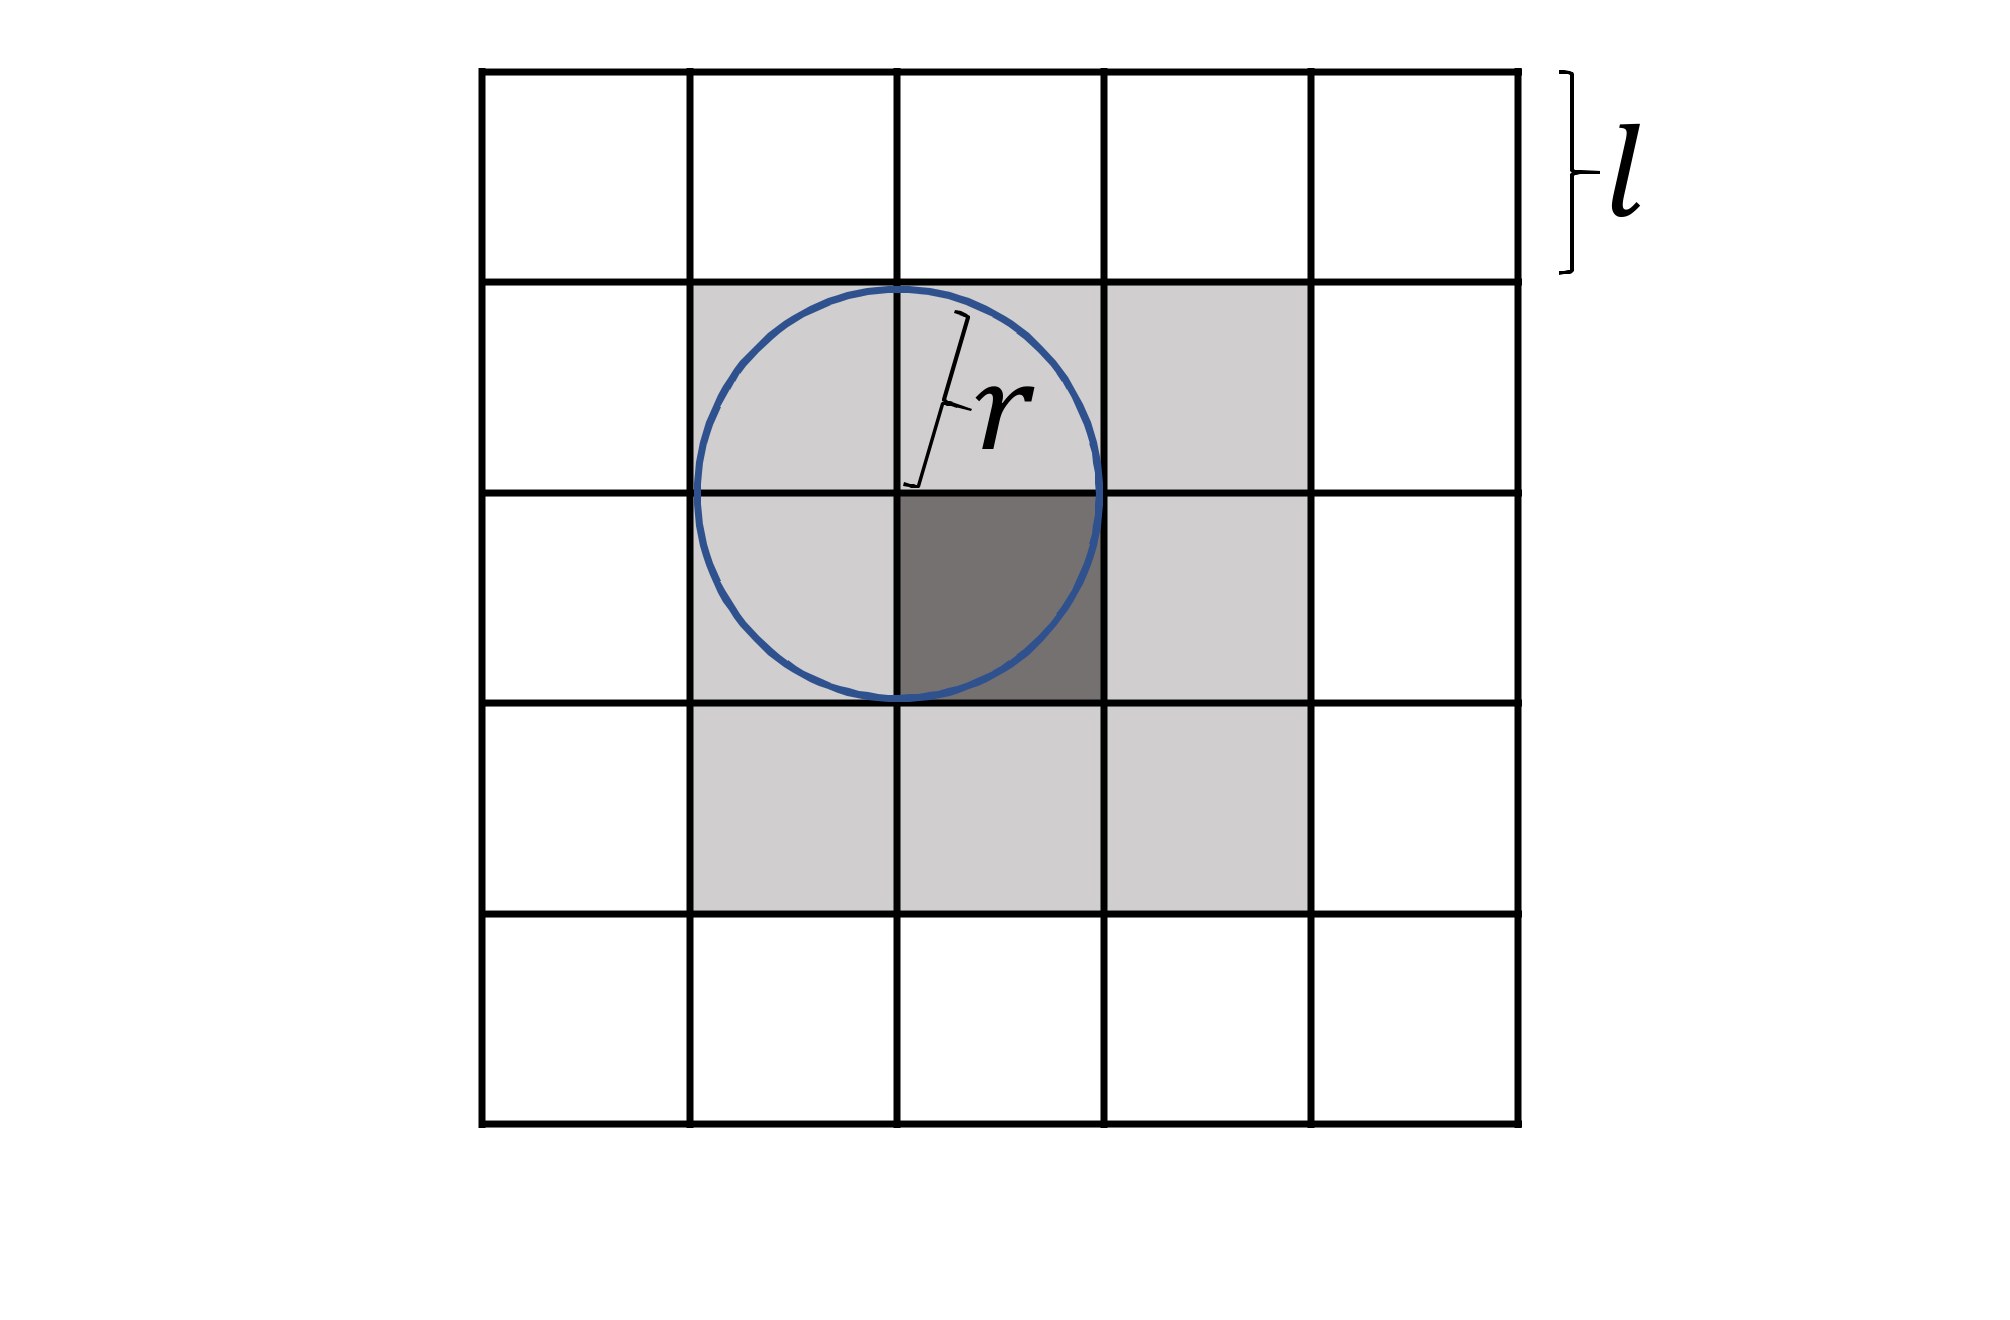
\includegraphics[height=2in]{figures/F53GridSizeForStillNodes.png}
  \caption{Grid Size For Still Nodes} 
  \label{fig:F53GridSizeForStillNodes} %% label for entire figure 
\end{figure}


\subsection{ Mobile Nodes}

\noindent The problem is a bit more complicated if nodes are moving. Assuming that we want to calculate all-pairs connections at $t_1$, first, we draw grids at time $t_0$, so that we know which grid is a node in at $t_0$. Instead of $t_0$, we want to get connections at $t_1$. In this case, the length $l$ might not equal to the radius threshold $r$.

Suppose that we have two nodes $u$ and $v$, and their distance is $d_1$ at $t_1$. Since the maximum speed of nodes is $S$, their distance $d_0$ at $t_0$ satisfies
\[max\left\{0,d_1-2\delta \right\}\le d_0\le d_1+2\delta \] 
where $\delta =S\left|t_1-t_0\right|$. When $d_1\le r$, these two nodes are connected at $t_1$, then $d_0$ must satisfy $0\le d_0\le r+2\delta $. If they are in the same or adjacent grids at $t_0$, as shown in Figure \ref{fig:F54LengthofGrid}. We have $l=r+2\delta $, so that $\mathrm{\forall }d_0\in \left[0,r+2\delta \right]$: $d_0\le l$. In other words, there is no grid between two nodes at $t_0$. 

\begin{figure} [hbtp]
  \centering 
  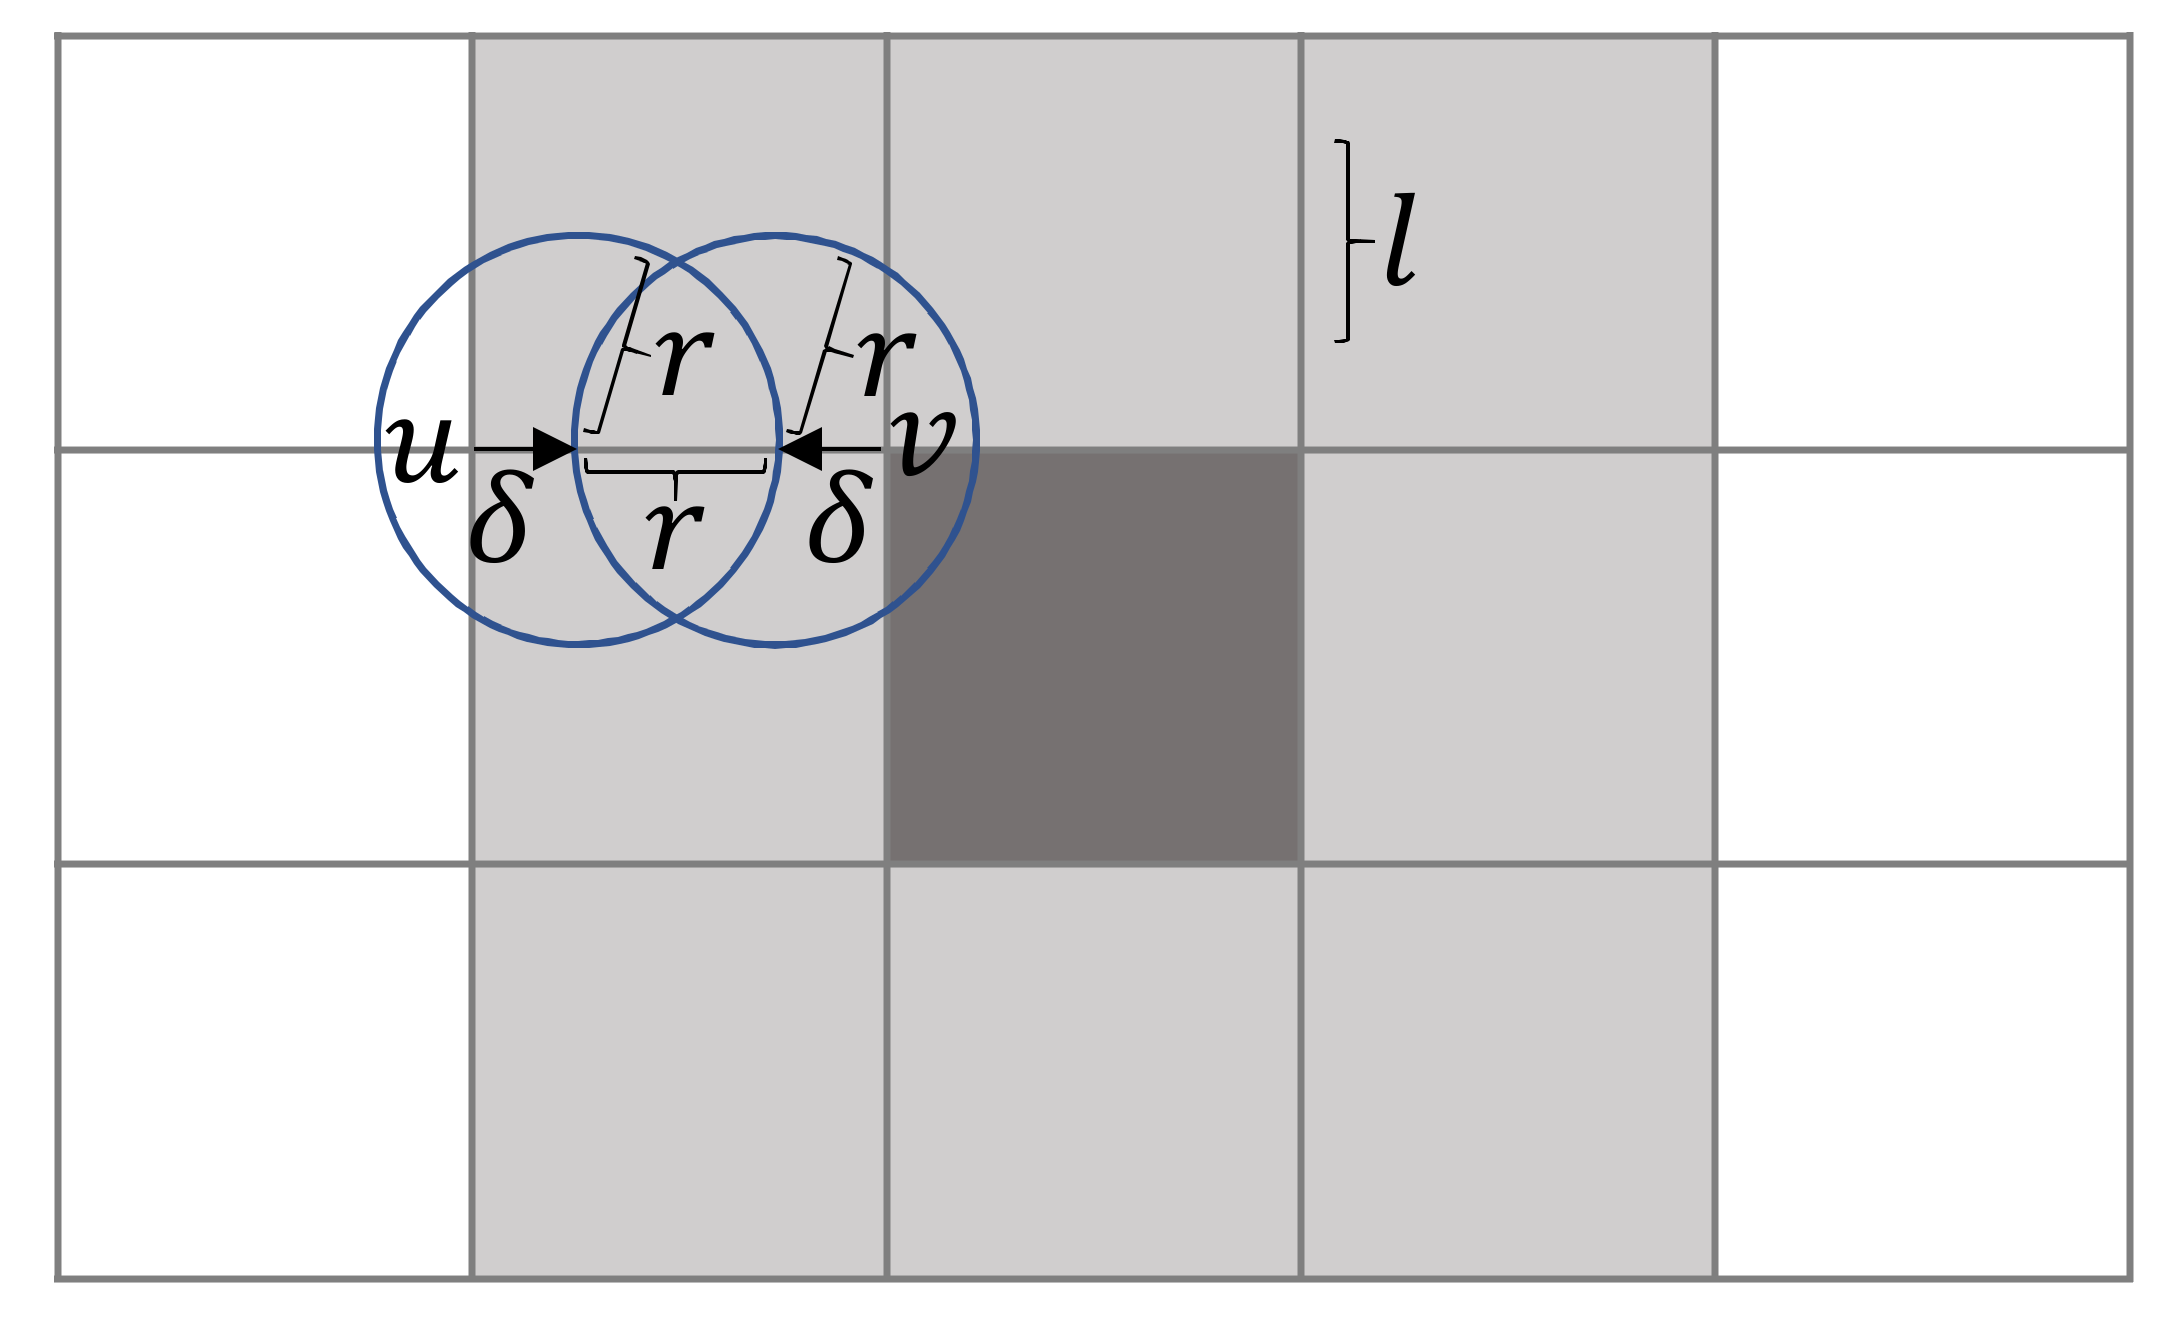
\includegraphics[height=2in]{figures/F54LengthofGrid.png}
  \caption{Length of Grid} 
  \label{fig:F54LengthofGrid} %% label for entire figure 
\end{figure}

\subsection{Complexity}

\noindent The complexity of drawing grids is $O\left(\frac{9n^2\times l^2}{2\times h\times w}\right)$, while that of checking connections is $\mathrm{O}\left(\frac{9n^2\mathrm{?}l^2}{2\mathrm{?}h\mathrm{?}w}\right)$, so the checking part is much more expensive than the drawing part. Since $l=r+2\delta =r+2S\left|t_1-t_0\right|$, the checking part achieves its best performance when $t_1-t_0=0$, then its complexity is $O\left(\frac{9n^2\times r^2}{2\times h\times w}\right)$. That is equal to the complexity when nodes are stationary.
















